\documentclass[a4]{scrartcl}

\usepackage[ngerman]{babel}
\usepackage[utf8]{inputenc}
\usepackage{mathtools}
\usepackage{amsmath}
\usepackage{amssymb}
\usepackage{geometry}
\usepackage{scrpage2}
\pagestyle{scrheadings}
\clearscrheadfoot


\geometry{
  paper=a4paper, % Change to letterpaper for US letter
  top=2cm, % Top margin
  bottom=1.5cm, % Bottom margin
  left=2cm, % Left margin
  right=3cm, % Right margin
  %showframe, % Uncomment to show how the type block is set on the page
}

\ohead{\\
Pina Kolling}

\setlength{\parindent}{0em}

\begin{document}


\section*{Vorlesung 2}

\textbf{Modelle}:
\begin{itemize}
    \item Reduktion von Komplexität
    \item \textbf{IST-Modell}: \\
    Abbild der realen Welt
    \item \textbf{SOLL-Modell}: \\
    Zukünftige Möglichkeiten
\end{itemize}

\textbf{Geschäftsprozessmodellierung}:
\begin{itemize}
    \item Erhöhung der Transparenz von Prozessen und Beziehungen innerhalb eines Unternehmens
    \item Erkennen von Zusammenhängen in betrieblichen Abläufen
    \item Erklärung der Funktionsweise des Unternehmens
    \item Erleichterung der Kommunikation im Unternehmen
    \item Grundlage zur Prozessoptimierung
    \item Einsatz zur Darstellung und Analyse verschiedener Lösungen
\end{itemize}


\textbf{Referenzmodell}:
\begin{itemize}
    \item immaterielle Abbildung
    \item Allgemeingültigkeitsanspruch (Wahl einer adäquaten Abstraktion)
    \item Flexibilität: Veränderungen mit geringem Aufwand durchführen
\end{itemize}
 \ \\
 
\textbf{Architektur integrierter Informationssysteme (ARIS)}:
\begin{itemize}
    \item Architekturmodell zur Gestaltung einzelner Informationssysteme
    \item Vorgangskettenmodelle betrieblicher Bereiche
    \item ARIS umfasst 4 Schichten: 
    \begin{itemize}
        \item Daten 
        \item Funktionen
        \item Steuerung
        \item Organisation
        \item ARIS umfasst 3 Entwicklungsstufen
        \begin{itemize}
            \item Fachkonzept
            \begin{itemize}
                \item Ausgangspunkt für Umsetzung von Betriebswirtschaft in Informationstechnik
            \end{itemize}
            \item DV-Konzept (Datenverarbeitung)
            \begin{itemize}
                \item Übertragung der Begriffswelt von Fachkonzept in DV-Konzept
            \end{itemize}
            \item Implementierung
            \begin{itemize}
                \item Übergang in Programmcode
            \end{itemize}
        \end{itemize}
    \end{itemize}
\end{itemize}

\newpage
\textbf{Ereignisgesteuerte Prozessketten (EPK)}:
\begin{itemize}
    \item Startereignis \& Endereignis
    \item Modellierungselemente Ereignis \& Funktion
    \item Operatoren AND, OR, XOR
\end{itemize}



\begin{center}
    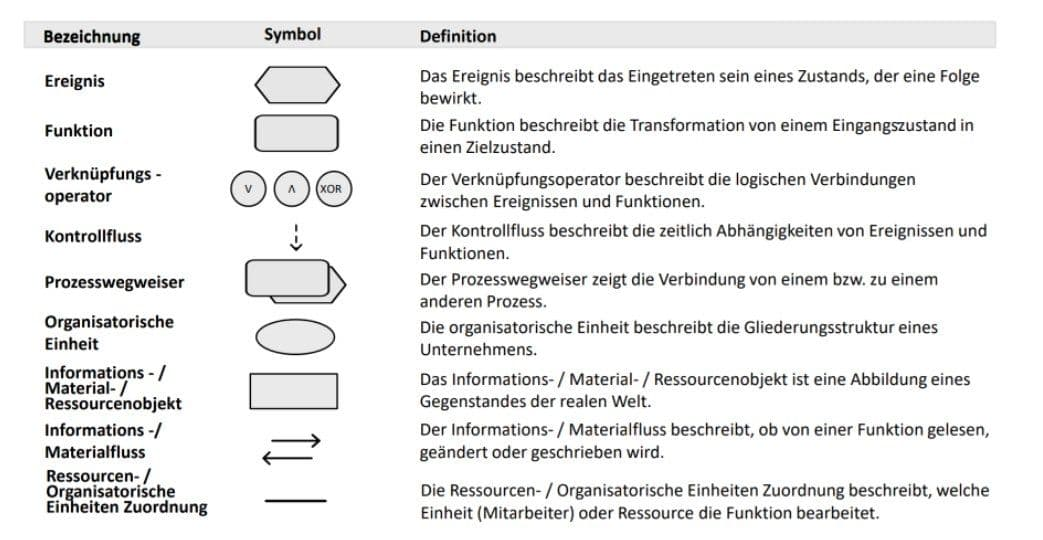
\includegraphics[width=19cm]{digi2.jpg}
\end{center}

\begin{itemize}
    \item EPK braucht mind. 1 Startereignis (oder Prozessschnittstelle)
    \item EPK braucht mind. 1 Endereignis (oder Prozessschnittstelle)
    \item nach Ereignis folgt Funktion oder Konnektor (Ausnahme: Endereignis)
    \item nach Funktion folgt Ereignis oder Konnektor
    \item jede Funktion hat genau eine ausgehende Kante
    \item jedes Ereignis hat genau eine eingehende und eine ausgehende Kante (Ausnahme: Start- und Endereignis)
    \item Konnektor hat entweder mehrere eingehende und genau eine ausgehende Kante oder genau eine eingehende und mehrere ausgehende Kanten
\end{itemize}

\newpage

\textbf{$\alpha$-Algorithmus}: \\

Muster in Geschäftsmodelle übersetzen

\begin{center}
    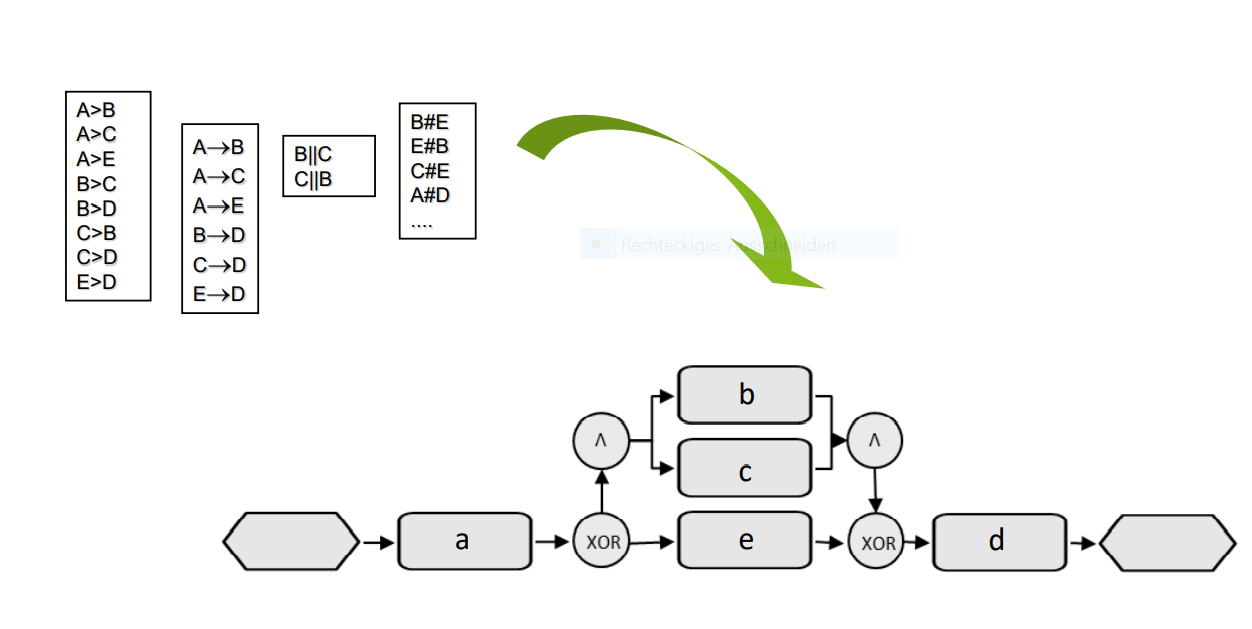
\includegraphics[width=18cm]{digi3.png}
\end{center}

\begin{center}
    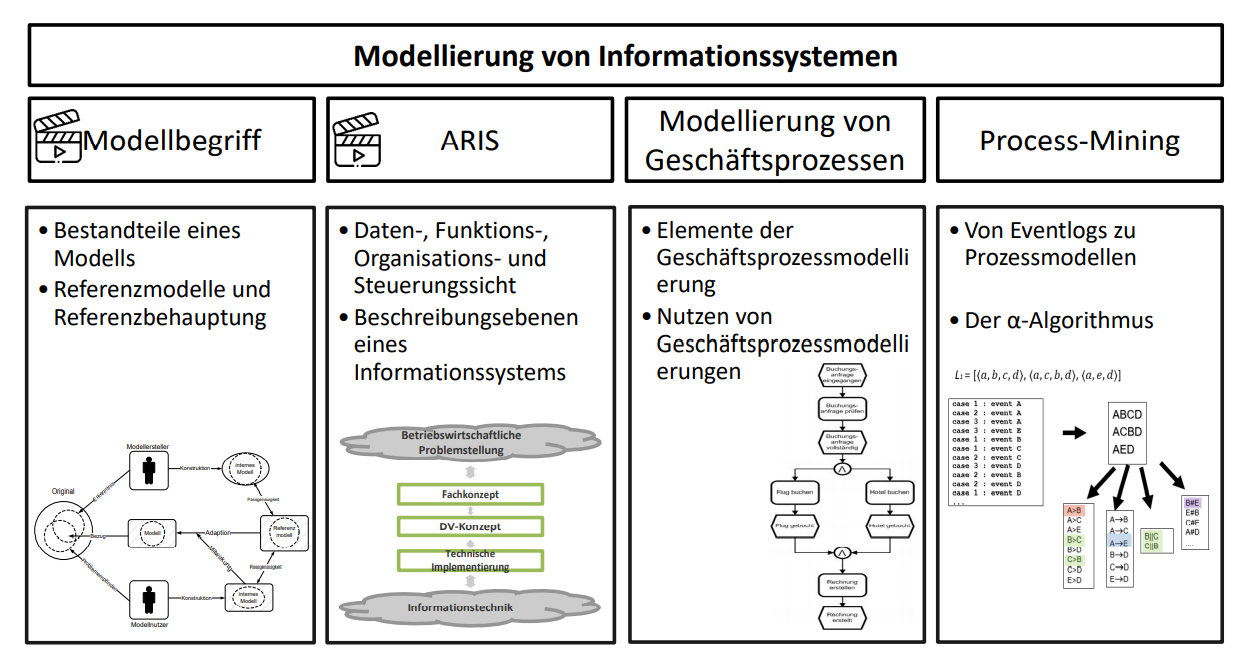
\includegraphics[width=18cm]{digi4.png}
\end{center}


\end{document}